\chapter{Methodology}
\label{ch:method} % Label for method chapter

\section{Research Design}

This study employs an experimental research design to develop and evaluate a routing system for existing large language model interfaces. The approach draws from both software engineering methodologies and machine learning research practices to create a systematic framework for development and testing. The research follows an iterative development methodology, beginning with the selection of a foundational NLI and progressing through the creation of increasingly sophisticated routing mechanisms. The ultimate goal is to produce a modular, extensible, and user-friendly Python library that can be integrated into various AI applications.

The methodology consists of eight distinct phases:

\begin{enumerate}
    \item Base NLI model selection
    \item System Architecture Design
    \item Generic Router prototype development
    \item Library Development And Architecture Design
    \item Evaluation framework creation
    \begin{enumerate}
        \item Automated Testing Script
        \item User Interaction CLI Tools
    \end{enumerate}
    \item Synthetic dataset generation (for testing)
    \item Plugin integration with existing AI systems
    \item Fine-tuning of base NLI model
\end{enumerate}

Each phase builds upon the previous ones, with continuous evaluation and refinement throughout the process. This iterative approach allows us to incorporate findings from earlier stages into subsequent development, creating a feedback loop that strengthens the overall system design.

\section{Selection of the Base NLI Model}

The initial phase involves selecting an appropriate foundation model and model architecture to serve as the cognitive engine for the routing system. This selection process considers several critical factors that directly impact the viability and performance of the resulting system.

We evaluated possible models against the following criteria:

\begin{itemize}
    \item \textbf{Classification Performance:} The model must demonstrate strong capabilities in text classification and categorisation tasks.
    \item \textbf{Inference Speed:} Given that routing decisions must occur with minimal latency to maintain system responsiveness, we established maximum acceptable response time thresholds based on human perception studies. Models exceeding these thresholds were eliminated from consideration regardless of their performance on other metrics.
    \item \textbf{Licensing Considerations:} Only models with permissive licensing terms suitable for both research and potential commercial applications were considered.
\end{itemize}

\begin{quote}
    For the experimental evaluation, we selected the open weights model: \texttt{facebook/\newline bart-large-mnli}.
\end{quote}

This model was selected for its strong performance on zero-shot classification tasks, particularly in the context of NLI; BART-Large-MNLI is a transformer-based model that has been pre trained on a large corpus of text and fine-tuned for NLI tasks, making it well suited for the routing system's requirements. The model's architecture allows it to effectively understand and classify complex prompts, making it an ideal candidate for the routing system \cite{lewis2019bartdenoisingsequencetosequencepretraining}. 

Some of the key features of the BART-Large-MNLI model include:

\begin{itemize}
    \item \textbf{Transformer Architecture:} BART-Large-MNLI is based on the transformer architecture, which has proven to be highly effective for a wide range of natural language processing tasks. This architecture allows the model to capture complex relationships between words and phrases in text, making it well-suited for understanding and classifying prompts.
    \item \textbf{Pre-trained on Large Datasets:} The model has been pre-trained on a large corpus of text, enabling it to leverage a wealth of knowledge and context when processing prompts. This pre-training helps the model generalise well to various tasks and domains.
    \item \textbf{Fine-tuned for NLI Tasks:} BART-Large-MNLI has been specifically fine-tuned for natural language inference tasks, which involve determining the relationship between a premise and a hypothesis. This fine-tuning makes the model particularly adept at understanding the nuances of language and context, allowing it to classify prompts effectively.
\end{itemize}

\newpage
\section{System Architecture}
\label{sec:system_architecture}

The architecture of the entire system is designed for the routers to sit between the user and the LLMs. The library is designed to be modular, allowing for easy integration with existing AI chat systems. In the following sections, I will describe the architecture of the system as a whole, and then the individual components of the system. The architecture is designed to be modular, allowing for easy integration with existing AI chat systems. The system should be designed to be extensible, allowing for easy addition of new models and tools in the future.


\subsubsection{Overview of the Routing Architecture}

Both the Model Router and Tool Router are designed use the same base structure, where the user prompt is passed to the router library, which then based on the prompt and the routing mechanism, selects the appropriate model or tool from the list of available models or tools. The selected model or tool is then used to invoke the model or tool and return the result to the user. 

\begin{figure}[H]
    \centering
    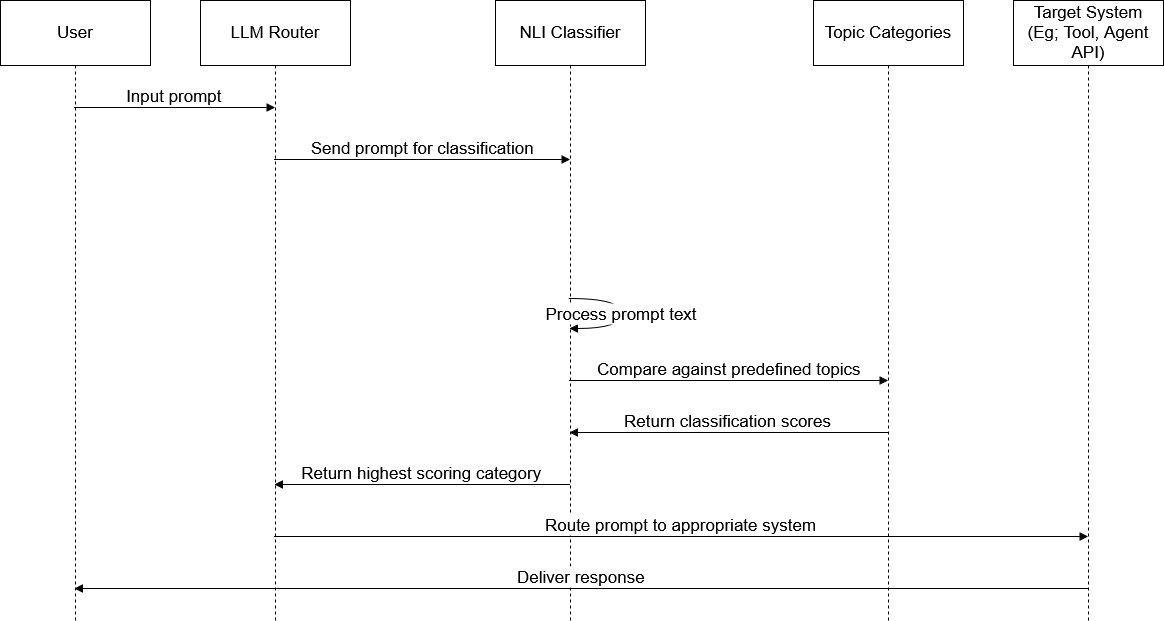
\includegraphics[width=1\textwidth]{figures/seq-digram.drawio.png}
    \caption{Sequence Diagram}
    \label{fig:seq_diagram}
\end{figure}


\textbf{NLI classification} uses a zero shot approach, where the prompt is treated as the \textit{premise} and the model or tool description is treated as the \textit{hypothesis}. The NLI model then scores each hypothesis against the premise, and returned. The model or tool with the highest score is withing a set threshold is selected and top n is returned.
\newline
In the figure above, the NLI model is used to classify the prompt into a category, from a list of categories which is then returned back to the library with a confidence score. The library then selects the model or tool with the highest score and based on the logic of the router, returns the model or tool to be used.
\newline
For example, if the user prompt is \textit{"Can you write a Python script to calculate the Fibonacci sequence?"}, with hypothesis being a list of: \textit{"Python script", "Email", "Mathematical calculation"} should return the Python script as the most relevant model with a confidence score.




\subsubsection{Model Router: Intelligent Selection of Processing Engines}

The Model Router serves as the first decision layer in our system, determining which language model should process the incoming prompt. This critical routing decision is based on multiple factors including the prompt's domain, complexity, and specific requirements. The Model Router can operate in three increasingly sophisticated modes:


\begin{figure}[H]
    \centering
    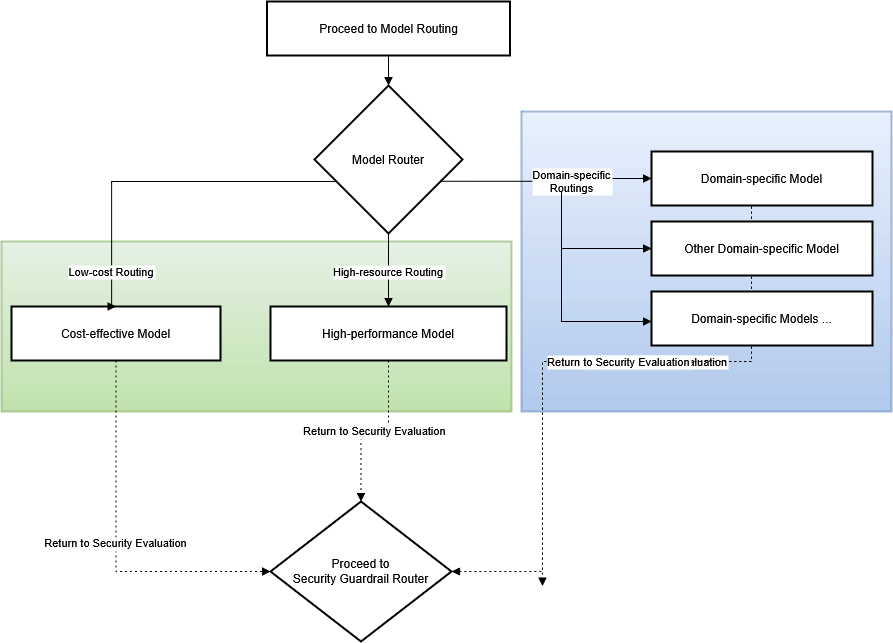
\includegraphics[width=1\textwidth]{figures/model-router.png}
    \caption{Model Router}
    \label{fig:model_router}
\end{figure}


\textbf{Mode 1: Cost-Performance Optimisation (Green)}


% \begin{figure}[H]
%     \centering
%     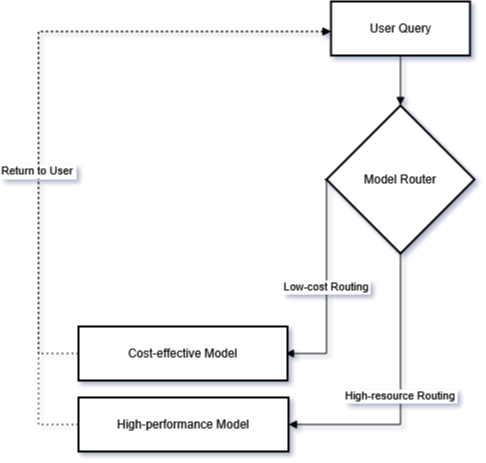
\includegraphics[width=0.5\textwidth]{figures/model-compx-router.drawio.png}
%     \caption{Simple Complexity Router}
%     \label{fig:simple_complexity_router}
% \end{figure}


In its simplest configuration, the Model Router functions as a binary decision maker (as shown in this paper \cite{lmsysroutellm}), choosing between:

\begin{itemize}
    \item \textbf{Cost effective models}: Smaller, more efficient models with lower computational requirements, suitable for straightforward queries or scenarios with resource constraints.
    \item \textbf{High performance models}: More capable but resource intensive models reserved for complex reasoning, creative tasks, or specialised knowledge domains.
\end{itemize}

This mode optimises resource allocation by matching prompt complexity to the appropriate level of model capability, ensuring efficient use of computational resources while maintaining response quality.

\textbf{Mode 2: Domain Specialisation (Blue)} 

In this more advanced configuration, the Model Router selects from an array of domain specialised models, each trained or fine tuned for excellence in particular knowledge areas. For example:

\begin{itemize}
    \item Code specialised models for programming tasks.
    \item Medical models for healthcare queries.
    \item Legal models for questions about law and regulations.
    \item Mathematical models for computational and quantitative problems.
\end{itemize}

This approach leverages the strengths of specialised training to deliver superior results in specific domains compared to general purpose models.

\begin{figure}[H]
    \centering
    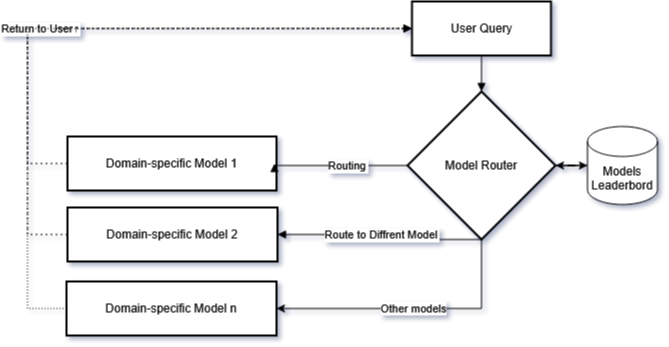
\includegraphics[width=0.5\textwidth]{figures/model-router.drawio.png}
    \caption{Domain Specialised Model Router}
    \label{fig:domain_specialised_model_router}
\end{figure}

\textbf{Mode 3: Hybrid Routing with Cascading Filters}

\begin{figure}[H]
    \centering
    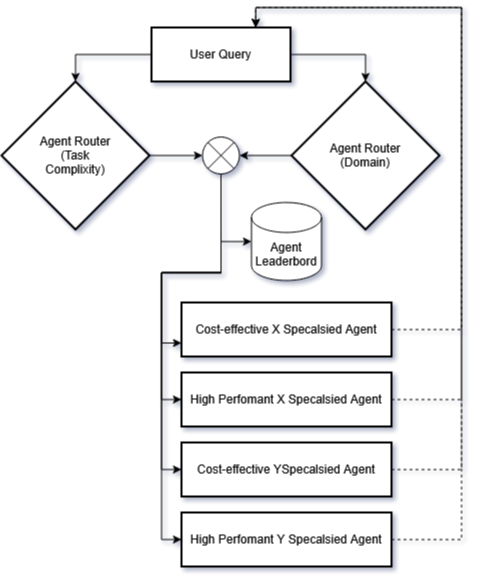
\includegraphics[width=0.5\textwidth]{figures/hybrid-agent-router.drawio.png}
    \caption{Hybrid Model Router}
    \label{fig:hybrid_model_router}
\end{figure}

A More sophisticated implementation combines the previous approaches into a comprehensive routing strategy. In this configuration, the system:

\begin{enumerate}
    \item \textbf{Domain Identification}: The system first evaluates the prompt against a set of predefined domain categories to determine whether specialised knowledge is required. This ensures that prompts are routed to models with relevant domain expertise when necessary.
    \item \textbf{Complexity Assessment}: Next, the prompt is analysed for complexity factors such as ambiguity, required reasoning depth, or expected response length to determine the appropriate performance tier within the identified domain.
    \item \textbf{Model Selection}: Finally, the system selects the optimal language model by consulting a lookup table or database. This table maps domains and complexity tiers to models that best balance domain specific expertise with computational efficiency and resource constraints.
\end{enumerate}

This hybrid approach leverages the strengths of both domain aware routing and resource optimisation, ensuring that each prompt is handled based on its content and requirements, while also matching it to models that can deliver high quality results within the available computational resources.

\begin{figure}[H]
    \centering
    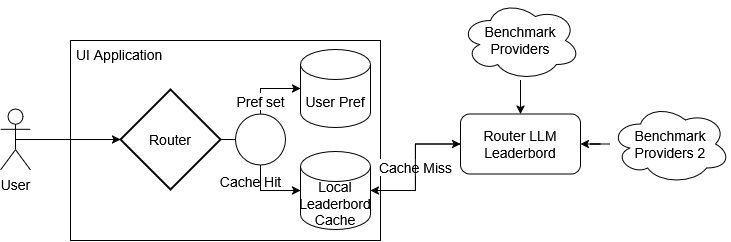
\includegraphics[width=0.7\textwidth]{figures/user-dig.drawio.png}
    \caption{Leaderboard based Model Selection}
    \label{fig:user_digram}
\end{figure}

To facilitate this process, resources such as a global; Vellum LLM leaderboard\footnote{\url{https://www.vellum.ai/llm-leaderboard}} or the Hugging Face Open LLM Leaderboard\footnote{\url{https://huggingface.co/spaces/open-llm-leaderboard/open_llm_leaderboard}} can be consulted. These leaderboards provide comprehensive, up to date benchmarking data on a wide array of language models and can inform model selection by considering multiple variables, such as:

\begin{itemize}
    \item \textbf{Average Score Across Benchmarks}: Selecting models based on their overall performance across a suite of standard benchmarks.
    \item \textbf{Instruction-Following Ability (IFEval)}: Prioritising models that excel at following user instructions accurately and coherently.
    \item \textbf{Big Bench Hard (BBH)}: Evaluating models on a collection of challenging tasks across domains, such as language understanding, mathematical reasoning, and common sense/world knowledge.
    \item \textbf{Mathematics Aptitude Test of Heuristics (MATH)}: Identifying models with superior mathematical reasoning abilities.
    \item \textbf{Environmental Impact}: Factoring in models with lower carbon dioxide emissions for greener operations.
\end{itemize}

In the following subsubsection, I will expand on how such a repository of could be serverd where 

\subsubsection{Advanced Model Routing Using Multiple Variables}

Model routing can be further enhanced by incorporating a multi variable lookup equation, enabling more nuanced and dynamic decision making. For instance, by adopting a hybrid routing strategy with cascading filters (as in Mode 3), the system can sequentially apply filters based on domain, complexity, instruction following capability, benchmark scores, and sustainability metrics. For example, the system could use a weighted scoring system with:

\begin{enumerate}
    \item \textbf{User's Previous Scoring}: The system can consider the user's historical ratings of models for specific domains, allowing for personalised routing based on past interactions.
    \item \textbf{Other Users' Scoring}: The system can aggregate ratings from other users to identify models that are generally well received in specific domains.
    \item \textbf{Average Score Across Benchmarks}: The system can use the average score across various benchmarks to evaluate model performance objectively.
\end{enumerate}

Furthermore, using a tagging and filtering system, the Model Router can dynamically adjust based on users requirements. For example, if a user priffers a model with a lower carbon footprint, the system can filter out models that do not meet this requirement. This allows for a more tailored and user centric experience, where the Model Router can adapt to individual preferences and priorities. This flexible approach ensures that each prompt is handled by the model most suited to its unique requirements, maximising both performance, resource efficiency and user satisfaction.


\[
\text{Score}_{m,t} = w_1 \cdot s^{\text{user}}_{m,t} + w_2 \cdot \overline{s}^{\text{others}}_{m,t} + w_3 \cdot s^{\text{benchmark}}_{m,t} + w_4 \cdot s^{\text{sustainability}}_{m} \cdot \delta_{\text{sus}}
\]

\text{where:}
\begin{align*}
&\text{Score}_{m,t} \quad\quad = \text{Total weighted score for model } m \text{ on topic } t \\
&s^{\text{user}}_{m,t} \quad = \text{User's score for model } m \text{ on topic } t \\
&\overline{s}^{\text{others}}_{m,t} = \text{Average score of other users for model } m \text{ on topic } t \\
&s^{\text{benchmark}}_{m,t} = \text{Benchmark score for model } m \text{ on topic } t \\
&s^{\text{sustainability}}_{m} = \text{Sustainability score for model } m \\
&w_1, w_2, w_3, w_4 = \text{Respective weights for each term} \\
&\delta_{\text{sus}} =
  \begin{cases}
    1 & \text{if user enabled sustainability} \\
    0 & \text{otherwise}
  \end{cases}
\end{align*}



\noindent
    \textbf{Interpretation:} \\
    This equation computes a weighted sum of model quality and preference indicators. Sustainability can be seamlessly included or omitted. The model with the highest score is selected for processing the prompt for that specific topic.
    
\subsubsection{Integration and Information Flow}

The complete system operates as a seamless processing pipeline:

\begin{enumerate}
    \item A user prompt enters the system.
    \item The Model Router evaluates the prompt's domain and complexity requirements.
    \item Based on this evaluation, the appropriate model is selected.
    \item The selected model begins processing the prompt.
    \item Concurrently, the Tool Router identifies any external tools required.
    \item If tools are needed, the model interacts with them via function calling.
    \item The integrated results from both model processing and tool outputs are combined.
    \item A comprehensive response is returned to the user.
\end{enumerate}

This architecture enables sophisticated query handling that dynamically adapts to varying prompt requirements while maintaining system efficiency. By separating model selection from tool selection, the system achieves a high degree of flexibility and extensibility, allowing for independent optimisation of each component.

In this script, I set up a simple command line interface that allows users to input prompts and receive routing results. The script uses the \texttt{AgentRouter}, \texttt{ToolRouter}, and \texttt{Router} classes from the \texttt{llm\_routers} library to route the input prompt to the appropriate agents, tools, and complexity levels. The results are printed in a user friendly format.

For the demo script, I also added a signal handler to gracefully shut down the routers when the user interrupts the script (by pressing ctrl+C). This ensures that any resources used by the routers are properly released.



\subsubsection{Potential Use of the Router as a Security Mechanism}
\label{sec:router_security}

The router's natural language understanding capabilities could be leveraged to identify adversarial prompts, such as prompt engineering attempts, potential jailbreaking patterns, and anomalous tool usage requests. This could serve as a preliminary security mechanism, although comprehensive security features are outside the core scope of this research. This aspect represents a promising direction for future work, particularly as the field of LLM security continues to grow. I will not go into detail about this in this paper, but I will show how a simple security guard could be implemented for the library. The security guard would work similarly to the router, where the prompt is passed to the security guard before being passed to the other routers. Additionally, the security guard would also be invoked after the prompt is inferred to check if the prompt is safe to be passed back to the user essentially acting as a wrapper around the whole system. 

\begin{figure}[H]
    \centering
    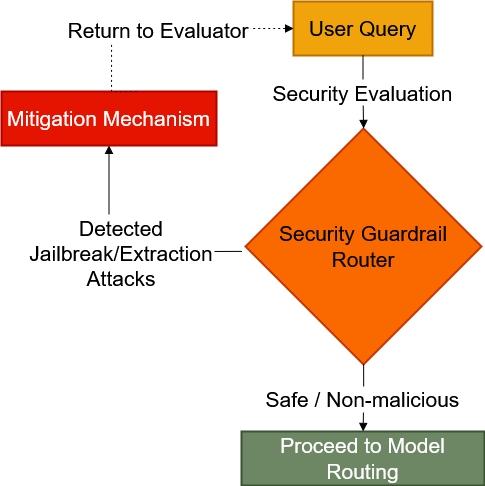
\includegraphics[width=0.4\textwidth]{figures/security-router.png}
    \caption{Security Guard}
    \label{fig:security_guard}
\end{figure}
%%%%%%%%%%%%%%%%%%%%%%%%%%%%%%%%%%%%







\section{Generic Prompt to Topic Router}
\label{sec:generic_router_dev}


Following model selection, The next phase involved developing a prototype router capable of classifying incoming prompts into predefined topic categories. This prototype served as the foundation for subsequent development efforts and allowed us to establish baseline performance metrics. The router is accessible via the \texttt{llm\_routers} library as the \texttt{Router()} class.

The Library is designed to have 3 main components one for each of the routing mechanisms. With a generic router for prompt to topic routing, a router for agent selection, and a router for tool selection.

\section{Python Library Development}
\label{sec:router_dev}

The main goal of this project is to develop a routing framework that can easily integrate with existing AI systems. Keeping this in mind, using the BART-Large-MNLI model as a base, and building upon the initial router prototype, I will develop a modular and extensible routing system that can be easily integrated into existing AI systems. Furthermore, the system will deployed as a Python library, allowing for easy installation and use in various applications.

Following strict software engineering principles, the library will follow software design patterns and best practices to ensure maintainability, extensibility, and ease of use. The main source code for the library is available on GitHub at \url{https://github.com/ru4en/llm_routers.git}. A CI/CD pipeline will be set up to ensure that the code is automatically deployed as a package that can be installed via pip. Linters and formatters will be used to ensure that the code is clean and easy to read asweell.


\subsection{Evaluation framework creation}
\label{sec:evaluation_framework}

A simple evaluation framework consisting of a set of automated tests and a command line tool for user interaction would also be a good addition so that users can easily test the library and see how it works. Aditionally, a set of synthetic datasets might be needed to test the library and see how it performs in different scenarios. Most likely, the datasets will be generated using a LLM such as Chat GPT or Claude.

\subsubsection{Plugin integration with existing AI systems}
\label{sec:plugin_integration}

To Finally demonstrate the effectiveness of the routing system, I will integrate it with an existing AI system. A good candidate for this is the Open Web UI, which is a popular open source project that provides a web interface for interacting with LLMs. Has a large community and is actively maintained and allows for easy integration with plugins written in Python.

\subsection{Fine-tuning of base NLI model}
\label{sec:fine_tuning}

Finally, I will also explore the possibility of fine-tuning the base NLI model with a dataset that is specifically designed for routing tasks. This will allow us to see if we can improve the performance of the model and make it more suitable for our specific use case. The fine-tuning process will involve training the model on a dataset that contains examples of prompts and their corresponding topics, allowing the model to learn the relationships between them.





